\label{sec:slits_section}
Другой составляющей аппаратной функции является функция углового распределения излучения в
экспериментальной схеме, определяемая геометрическими особенностями (размерами щелевых
коллиматоров и длинами оптических путей). Рассмотрим преобразование пучка рентгеновского
 излучения проходящего через систему щелевых коллиматоров.
\begin{figure}[H]
  \centering
  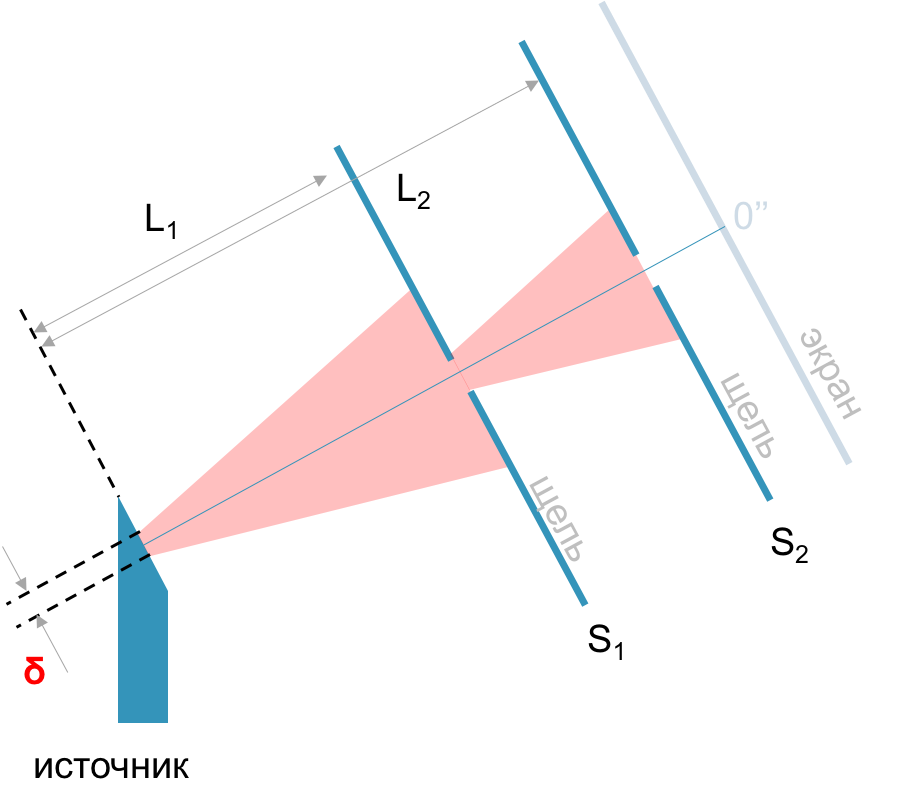
\includegraphics[width=0.6\textwidth]{images/for_slits.png}
  \caption{Схематичное изображение распространение рентгеновского пучка в
  системе с протяженным источником и двумя щелевыми коллиматорами}
  \label{ris:for_slits}
\end{figure}

На начальном этапе рассматривалась модель точечного источника излучения
 (протяженность источника $\delta = 0$).
В таком случае, интенсивность проходящего излучения будет определятся
одним щелевым коллиматором, которое является более узким из двух при пересчете в угловые
координаты. Например, для фиксированных расстояний между элементами $L_1 = 570$ мм, $L_2 = 1005$ мм,
 в случае одинаковых линейных размеров щелей и точечного
источника, интенсивность будет определяться более удаленным щелевым коллиматором, и
распределение интенсивности принимает вид представленный на рис. \ref{ris:sourc_map_a}. Если источник является
протяженным ($\delta \neq 0$), то угловое распределение интенсивности принимает более сложный вид,
 как показано на рис. \ref{ris:sourc_map_b}.


\begin{figure}[H]
  \centering
  \subfloat[]{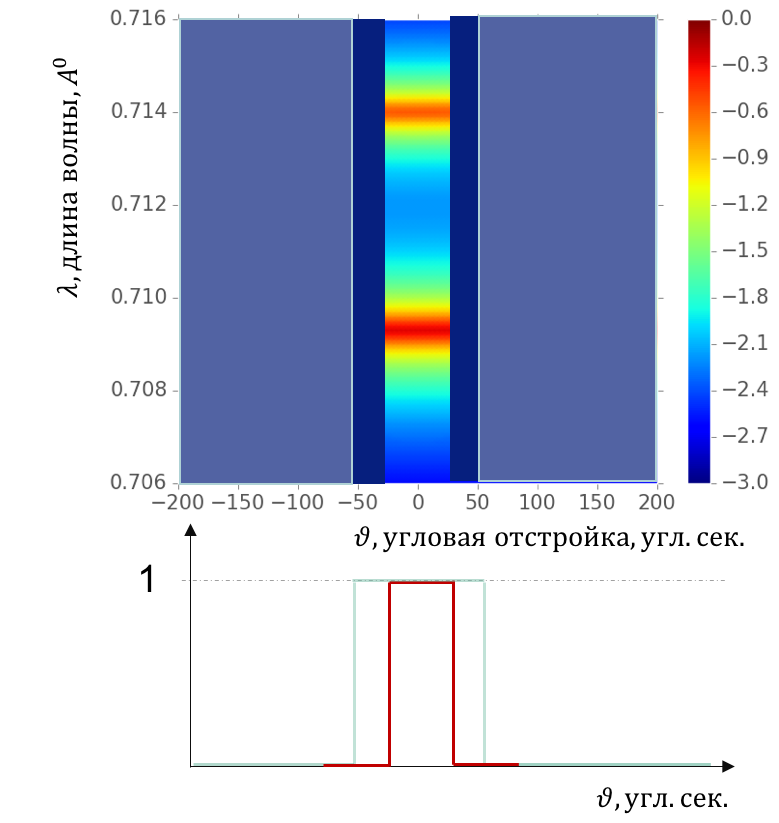
\includegraphics[width=0.5\textwidth]{images/point_sourc_map.png}\label{ris:sourc_map_a}}
  \hfill
  \subfloat[]{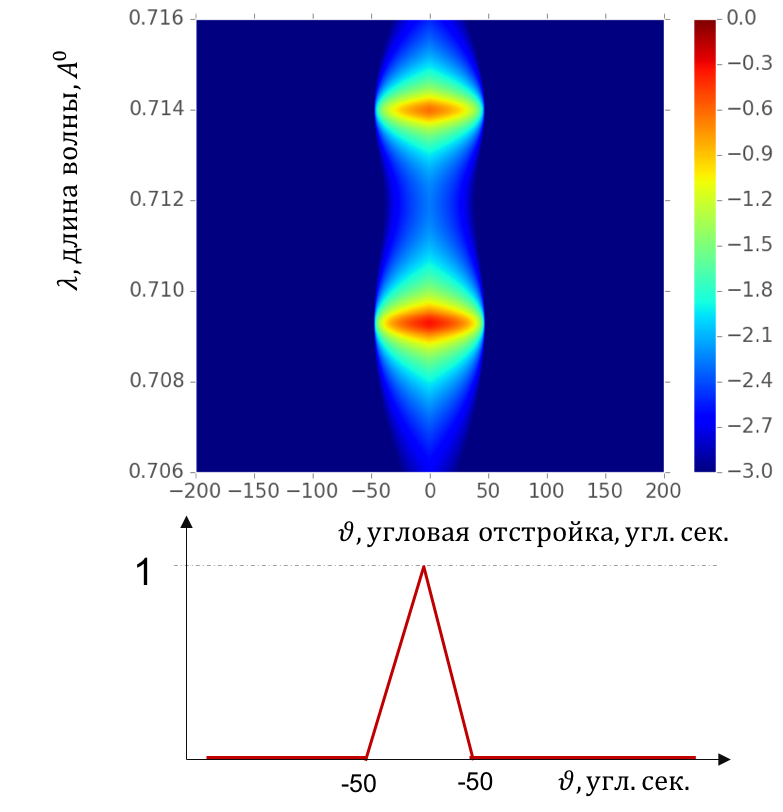
\includegraphics[width=0.5\textwidth]{images/wide_sourc_map.png}\label{ris:sourc_map_b}}
  \caption{Спектрально-угловое распределение излучения в системе двух щелей для различных типов источника: точечного (a)
  и протяженного ($\delta = 0.2$ мм) (b)}
  \label{ris:sourc_map}
\end{figure}

Необходимо отметить, что для описания дифракционного эксперимента имеет значение именно
спектрально-угловое распределение излучения, т.е. количество и энергия квантов, падающих под тем
или иным углом на кристалл. Данное распределение определяется соотношение площадей параллелограммов,
угол между боковой стороной и основанием которых соответсвует углу распространения излучения
(рис. \ref{ris:how_many_quants_use_parallelogr}).

\begin{figure}[H]
  \centering
  \subfloat[]{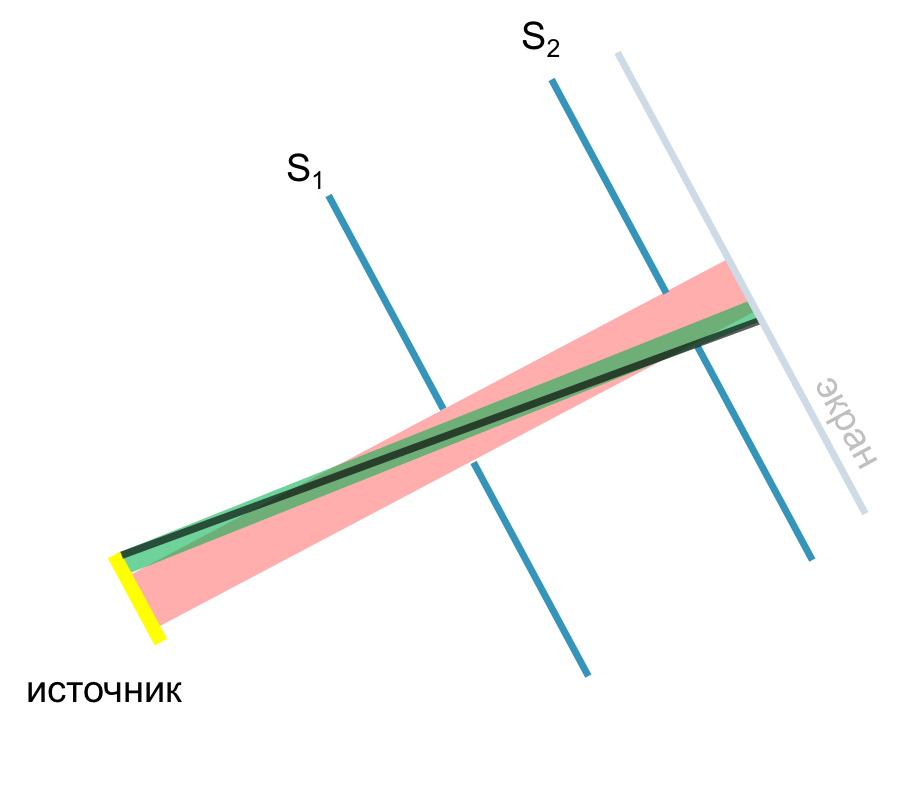
\includegraphics[width=0.45\textwidth]{images/how_many_quants_use_parallelogr_1.png}}
  \hfill
  \subfloat[]{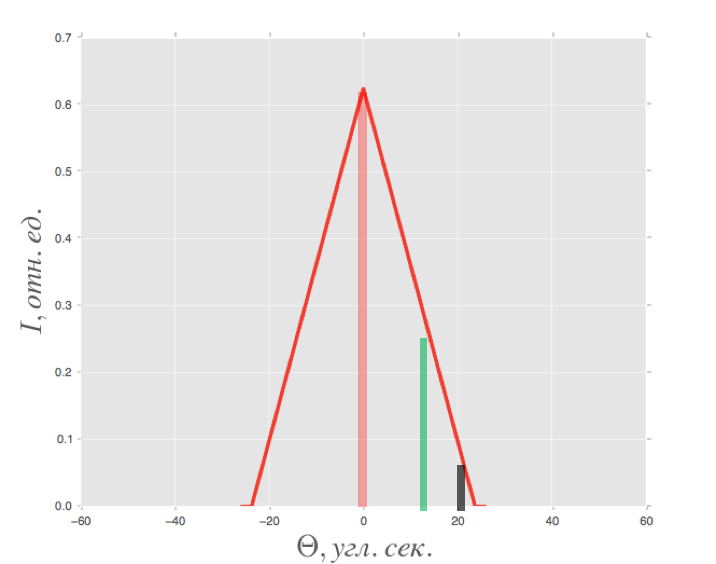
\includegraphics[width=0.45\textwidth]{images/how_many_quants_use_parallelogr_2.png}}
  \caption{Схематичное представление углового распределения излучения после
  прохождения системы щелевых коллиматоров. Пропускная способность системы
  щелей в определенном угловом направлении соответствующего параллелограмма (a).
   Интенсивность на экране, установленном после системы щелей для
   протяженности источника $\delta = 0.2$ мм (b)}
  \label{ris:how_many_quants_use_parallelogr}
\end{figure}
Более подробный расчет $g_S(\vartheta)$ представлен в Приложении 3.
На рис. \ref{ris:calc_slits_ability_res} представлены результаты расчета пропускной способности
системы двух щелей для некоторых параметров ренгенооптической схемы в приближении
 точечного источника ($\delta = 0$), в сравнении с протяженным ($\delta \neq 0$).

\begin{figure}[H]
 \centering
 \subfloat[]{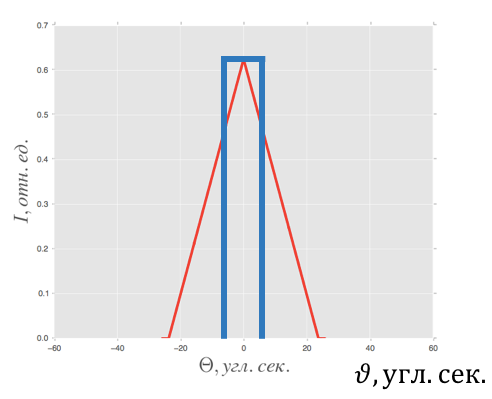
\includegraphics[height=6em]{images/calc_slits_ability_res_1.png}}
 \hfill
 \subfloat[]{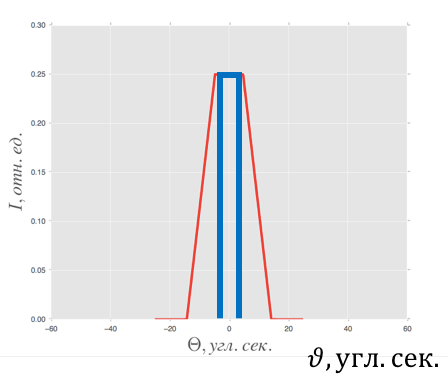
\includegraphics[height=6em]{images/calc_slits_ability_res_2.png}}
 \hfill
 \subfloat[]{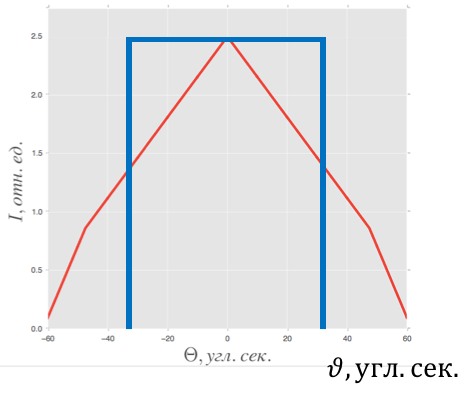
\includegraphics[height=6em]{images/calc_slits_ability_res_3.png}}
 \hfill
 \subfloat[]{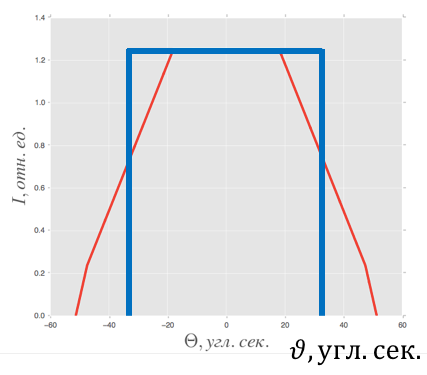
\includegraphics[height=6em]{images/calc_slits_ability_res_4.png}}
 \caption{Пропускная способность щелевых устройств в зависимости от угла распространения
 рентгеновского излучения. Расстояние до первой щели $L_1 = 570$ мм, до второй - $L_2 = 1005 $ мм.
 Размеры щелевых коллиматоров и протяженность источника:
   $S_1 = S_2 = 50$ мкм; $\delta = 0.2$ мм (a),
   $S_1 = 20$ мкм; $S_2 = 40$ мкм; $\delta = 0.2$ мм (b),
   $S_1 = 200$ мкм; $S_2 = 400$ мкм; $\delta = 0.2$ мм (c),
   $S_1 = 200$ мкм; $S_2 = 400$ мкм; $\delta = 0.1$ мм (d)}
 \label{ris:calc_slits_ability_res}
\end{figure}

Анализ рис. \ref{ris:calc_slits_ability_res} показывает, что перегиб  возникает вследствие переходного
процесса от точечного источника к бесконечному, т.е. на меньших углах плотность
излучения определяется ближайшей, а начиная с некоторого угла ограничивать пучок начинает
более удаленная щель.
 %\textcolor{mygreen}{НАРИСОВАТЬ РИСУНОК}(рис. ).
